\chapter{Approach}
In this chapter, we describe the approach of this thesis by presenting the main ideas to reach our goals for the simulation in section 4.1. In section 4.2, we present the architectural approach.

\section{Goals and Approaches}
\textbf{Realistic simulation:} The realism of the simulation is an important goal of the thesis. A more realistic simulation allows better testing because the simulation is more similar to the reality. Therefore more problems of reality can be simulated. The reality of the simulation has many different aspects. The first group of aspects belong to the realism of the sensor data. There are some sensors that are easy to simulate, such as distance sensors, bumpers and gyroscopes. Others, especially cameras, are more difficult to simulate realistically. The choice of Gazebo with ODE and Ogre for the visual appearance already allows us to simulate a wide range of sensors realistically. An other aspect for the realism is noise in the sensor data. For all metric sensors, we simulate this as Gaussian noise with the calculated value as mean and a configurable variance. The second group of aspects belong to the realism of the physical environment. Objects have to behave in the simulation and the reality in a similar way. This is especially important for robot movement and manipulation tasks. Here Gazebo with ODE also provides high realism out of the box. Nevertheless, it is important to find good physical parameters for the simulated objects. Examples of those parameters are the mass and coefficients of friction. An other important aspect of realism is that the simulation should not introduce new problems which do not occur in reality. Such a problem, which occurred in the development of the thesis, is that the simulation ran slower than the system time.\\
\textbf{Different levels of simulation:} Besides a simulation, which is so realistic as possible, it is also useful to test with a more abstract simulation. This allows testing the optimal case without sensor noise or without using low level components, such as localization, if those produce new errors or are not finished jet. To be able to simulate on different levels we use the multi-level abstraction approach presented in the chapter about related work~\cite{MultiLevelAbstraction}. We use multi-level abstraction for sensing and for actuating. How we use multiple abstraction levels is shown in the next section about the architecture.\\
\textbf{Compatibility with original robot software:} We want to achieve the goal that the robot software runs in the simulation in the same way as in reality. This is important because otherwise it would result in additional effort to keep the robot software in the simulation and in the reality running and this effort can cause more difference between simulation and reality. In the thesis, the simulation should use the same interfaces as the real components that are simulated. In Fawkes this is easy to achieve because the interfaces between components are well defined and components using an interface do not recognize whether the interface is provided by the simulation or a real component. \textcolor{red}{woerter zu oft wiederholt?}\\
\textbf{Efficient testing:} We want to make the use of the simulation as efficient as possible. To achieve this, we provide the following features. We provide scripts which automatically start the full simulation with all needed programs. Without this scripts, it would take much time. For a full simulation of an LLSF game, it is necessary to start Gazebo, the Refbox, a controlling Fawkes instance and, for the Robotinos, three times Fawkes, Roscore and Movebase\footnote{Movebase is the ROS program we currently use for navigation with collision avoidance.}. Each program-instance has to be started with correct parameters.  An other approach we use to increase the efficiency is the feature to load different configurations and setups. For example, the scripts provide the possibility to load the simulation with different numbers of Robotinos, abstraction levels and simulation environments. Loading different configurations for the robot software is a feature of Fawkes and useful for us. We also integrated this in the scripts. We also provide the possibility to draw objects into the simulation. This makes it easy to visualize the belief and intentions of a robot to identify mistakes or ways to improve the system~\cite{Visualization}.\\
\textbf{Multi-robot system evaluation:} An important part of this thesis is the evaluation of multi-robot systems. The features we already mentioned in the previous paragraph are here especially useful because the testing effort (e.g. to setup the simulation or analyzing the cooperation between robots) often scales with the number of robots. To evaluate the performance of the multi-robot system faster without having to observe the simulation all the time, we provide the possibility to run multiple simulation runs, in our case runs of LLSF games, automatically. With this feature, the simulation can run for example 20 times over night. To analyze the executed simulation runs, we keeps statistics of each run. For our LLSF domain, we keep the amount of achieved points with a detailed list of all actions which gave points at which time. These statistics can easily be extended by the amount of collisions between robots, waiting time for resource locks or other useful measurements. Sometimes it can happen that single simulation runs have a very different result. To find the reason for this result, we keep the log files of the run and also record the simulation itself. With this record, the simulation run can be reconstructed. The record contains the position and movements of all objects in the simulation. Here it is also useful to draw additional information, such as the localization of the robots, in the simulation to be able to analyze faults without having to look in the log files. The automated simulation runs also allow the comparison of different configurations of the multi-robot system. The automation script can be started with a number of configurations that are all tested. This can be useful for finding the best performing role combination or parameters such as thresholds.\\
\textbf{Expendability and flexibility:} An essential criterion of a good simulation is the expendability to adapt to future changes. On the one hand, there will be changes to the Carologistics Robotino and to LLSF. These changes have to be easy to implement in the simulation, otherwise the simulation would not remain useful. On the other hand, it is attractive to use the simulation also in other domains, such as RoboCup @Home. To achieve the expendability of the simulation, we provide a framework for simulated devices in Gazebo and Fawkes. Furthermore we concentrate on developing small modules that are exchangeable and reusable. In Gazebo, new modules can easily be added to the robot and world plugins. In Fawkes it is easy to implement a new plugin which provides the wanted features because the plugin can use the provided Gazebo aspect. In addition, a detailed documentation and example plugins allows other developers to easily extend the simulation. \textcolor{red}{TODO: wiki plugin dev!}. The simulation should also be flexible to adapt to small changes. Therefore we provide several configuration files for the simulation environment, the simulated objects and robots and the plugins for Gazebo and Fawkes. \textcolor{red}{Gazebo config}


\section{Architecture}

\subsection{Simulation}
\begin{figure}
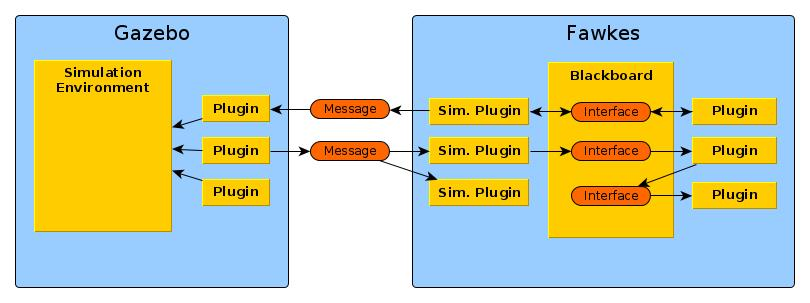
\includegraphics[width=\textwidth]{tabs/fawkes_gazebo}
\caption{Architecture of the simulation}
\label{fig:fawkes_gazebo}
\end{figure}
The basic structure of the simulation is shown in Figure~\ref{fig:fawkes_gazebo}. On the one side, there is the Fawkes robot software framework we want to run in the simulation. On the other side, there is the simulator Gazebo. Roughly, the simulation is composed of a simulation environment, which handles the physical and visual simulation of the environment based on defined world and models, and plugins associated to the world and all models with some kind of behavior. There are plugins instances for the sensors and actuators of each robot as well as plugins that control the world to, for example, set the machine lights. At this point, Fawkes can be seen as a composition of plugins, which are used on the real robot system, simulation plugins, which communicate with the simulation to exchange original sensor and actuator plugins, and the blackboard. The blackboard manages several interfaces which are used for communication between Fawkes plugins. The Fawkes simulation-plugins send actuator messages to the corresponding Gazebo plugins and receive messages from sensor-plugins in Gazebo. This architecture has the advantage to be flexible and extendable. To add a new sensor or actuator to the simulation, it is sufficient to create a Gazebo plugin for simulation and Fawkes simulation-plugin to provide the corresponding interface. Furthermore, the architecture is flexible enough to allow multi-level abstraction, see later subsection.


\subsection{Communication Fawkes-Gazebo}
\begin{figure}
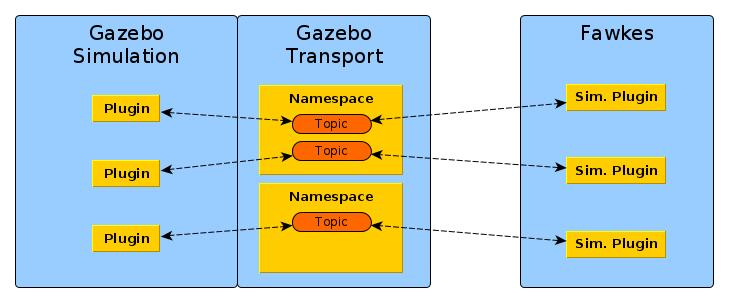
\includegraphics[width=\textwidth]{tabs/communication}
\caption{Communication between Fawkes and Gazebo}
\label{fig:communication}
\end{figure}
The communication between Fawkes and the Gazebo simulation has a specific structure to organize the distinction between the multiple robots and the different sensors and actuators. Figure~\ref{fig:communication} shows this structure. Fawkes simulation-plugins and Gazebo plugins communicate over a message-transport system. In our case, this system is embedded in the Gazebo Transport API. In the message-transport system, there are different nodes which act as communication channels. There is one node for each simulated robot and for the simulated world. The topics in a node represent what the messages, which are send on this topic, are about. Each plugin can listen to or send on the topics in a node. For example there are topics about laser data and motor commands. This architecture is extendable because it is easy to add new nodes or topics. It is flexible, because the communication through a topic in a node is a many-to-many relationship, and it is comfortable, because instances of plugins in different Fawkes instances can listen to the same topic and get data from different simulated robots because the plugins listen do different channels.


\subsection{Multi-level Abstraction}
\begin{figure}
\centering
\begin{subfigure}[b]{\textwidth}
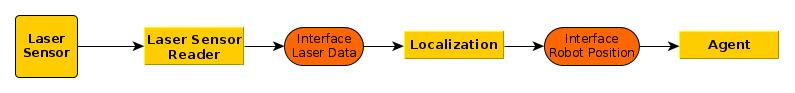
\includegraphics[width=\textwidth]{tabs/mla_hardware}
\caption{With real hardware}
\label{fig:mla_hardware}
\end{subfigure}
\begin{subfigure}[b]{\textwidth}
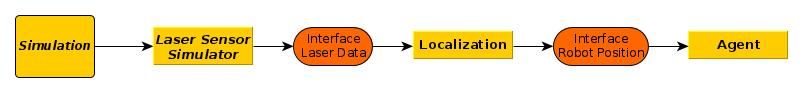
\includegraphics[width=\textwidth]{tabs/mla_sim_low}
\caption{With low level abstraction}
\label{fig:mla_sim_low}
\end{subfigure}
\begin{subfigure}[b]{\textwidth}
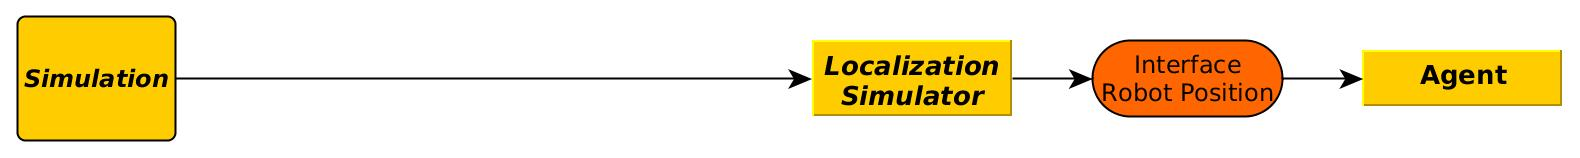
\includegraphics[width=\textwidth]{tabs/mla_sim_high}
\caption{With high level abstraction}
\label{fig:mla_sim_high}
\end{subfigure}
\caption{Example for multi-level abstraction}
\label{fig:mla}
\end{figure}
Figure~\ref{fig:mla} shows how multi-level abstraction fits in our simulation architecture. We choose a simple example about the localization with laser data. In Figure~\ref{fig:mla_hardware}, there is the system as it is used in the real application. There is the laser sensor hardware, a plugin which reads out the sensor and publishes the laser data in an interface, a localization plugin which uses the laser data interface to determine a robot position and to provide the position in an other interface. Then, the robot agent uses the position information from the interface. Figure~\ref{fig:mla_sim_low} shows the system in the simulation with low level abstraction. The hardware is replaced by the simulation and the laser sensor reader by simulation-plugin which gets the laser data from the simulation. This simulation-plugin provides the same interface as the original plugin. An other possibility with high level abstraction is shown in Figure~\ref{fig:mla_sim_high}. Here, the localization plugin is replaced by a simulation-plugin which simply looks up the position of the robot in the simulation and writes as in the interface. The agent can now be simulated with ground-truth position data and without use of the original localization plugin. An example for multi-level abstraction for actuators could be the movement of a robot. It is possible to simulate the motors with motor commands from an interface or the motion of the robot by applying the motion command in an interface directly to the simulated robot.
